\chapter{Requirements Engineering}

ISO/IEC/IEEE 29148-2011 {\em Systems and Software Engineering - Life Cycle Processes - Requirements Engineering}:
\begin{quote}
% function that mediates between the domains of the acquirer and supplier to establish and
%maintain the requirements to be met by the system, software or service of interest

\ldots is an \hl{interdisciplinary} process
concerned with discovering, eliciting, developing, analyzing, determining
 verification methods, validating, communicating, documenting, and managing requirements.
\end{quote}
\newslide

Glossary:
\begin{itemize}
  \item
    \structure{Requirement}: statement which translates or expresses a need and its associated constraints and conditions
     to solve a problem or to achieve an objective.
%
%\item
%  requirements elicitation: process through which the acquirer and the suppliers of a
%  system discover, review, articulate, understand, and
%  document the requirements on the system and the life cycle processes.
%
\item
  \structure{Stakeholder}: individual or organization having a right, share, claim, or interest in
  a system or in its possession of characteristics that meet their needs and expectations.
 Stakeholders include, but are not limited to, end users, end user organizations, supporters, developers,
producers, trainers, maintainers, disposers, acquirers, customers, operators, supplier organizations, accreditors, and
regulatory bodies.

%\item requirements validation:
%confirmation by examination that requirements (individually and as a set) define the right system as intended
%by the stakeholders
%
%\item
%  requirements verification: confirmation by examination that requirements (individually and as a set) are well formed
%NOTE
% This means that a requirement or a set of requirements has been reviewed to ensure the characteristics of
%good requirements are achieved.
%
%requirements management
%activities that ensure requirements are identified, documented, maintained, communicated and traced
%throughout the life cycle of a system, product, or service
%
\end{itemize}
\newslide
Tasks:
\begin{itemize}
\item \structure{Elicitation}:
 build an understanding of the problem that
 the software is required to solve. It is fundamentally a human activity and is where
 the stakeholders are identified and relationships established
between the development team and the customer.
  % Goals, Domain Knowledge, Stakeholders, Business Rules, Environment
\item \structure{Analysis}:
  detect and resolve conflicts between requirements,
  discover the bounds of the software and how
    it must interact with its organizational and operational environment,
 elaborate system requirements to derive software requirements.

% Classification (functional/non-functional), Priority, Scope, Volatility
%
%  Grundlegende Konkretisierung und Abgrenzung des Projektes, so dass 
%  dessen Inhalte und Ziele entscheidbar und planbar werden,
%%
%\item  Analyse des Anwendungsbereiches mit Erfassung aller wichtigen Anforderungen
%  an das Produkt
%
\item \structure{Architectural Design}: design the system structure with its components,
  their connections and interfaces.
  %%
  \newslide
\item \structure{Specification}: create a document that can be systematically reviewed,
  evaluated, and approved.

  Types:
\begin{itemize}
\item Stakeholder Requirements Specification
\item System Requirements Specification
\item Software Requirements Specification
\end{itemize}
%
%software requirements specification
%structured collection of the requirements (functions, performance, design constraints, and attributes) of the
%software and its external interfaces
%

\item \structure{Validation}:
  verify that a requirements document conforms to company standards
  and that it is understandable, consistent, and complete

\end{itemize}
%{\bfseries Requirements-Engineering}
%\begin{centering}
%\includegraphics[width=0.8\linewidth]{img/requirements-engineering}
%Elicitation $\longrightarrow$ Analysis $\longrightarrow$ Specification $\longrightarrow$ Validation
%\end{centering}
%
\newpage
%\ifslides
%\else
%Zu klärende Fragen:\\[2ex]
%\fi
\begin{boxedminipage}{\linewidth}
\begin{itemize}
\item {\bfseries Wer} ist involviert?\\ 
(Benutzerprofil, Projektbeteiligte, Zuständigkeiten, Organigramm)
\item {\bfseries Wie} ist die gegenwärtige Situation?\\
  (Geschäftsprozesse, ev. Probleme, Schwachstellen)
\item {\bfseries Wann} muss das System lauffähig sein?\\
 (Termine, Meilensteine)
\item {\bfseries Wo} wird das System installiert?\\
  (HW/SW-Umgebung)
\item {\bfseries Warum} ist eine Neuentwicklung notwendig?\\
  (Zielsetzungen, Nutzen, Risiken)
\item {\bfseries Was} muss das System leisten?\\
 (Funktionalität, Mengengerüst)
\item {\bfseries Welche} Einschränkungen sind zu berücksichtigen?\\ 
(Programmiersprachen, Zuverlässigkeit, Antwortzeiten, Speicherbedarf etc.)
\end{itemize}
\end{boxedminipage}
\newslide
\vspace{0.5cm}

Ergebnisse:
\begin{itemize}
\item Anforderungsspezifikation (Requirements Specification)
\item Projektplan
\end{itemize}
InformationsSourcen:
\begin{itemize}
\item Interviews, Workshops
\item Fachliteratur, Zeitungen, Zeitschriften, Handb"ucher, Lexika
\item Dokumente, Formulare, Arbeitsanweisungen, Vorschriften
\item Internet
\end{itemize}
%\newpage
%
%--------------------------------------------------------------------------
%\ifslides
\newpage
%\fi
%\kopf
\section{Non-Functional Requirements}
%       \addcontentsline{toc}{subsection}{Nichtfunktionale Anforderungen}
Alle Anforderungen, die nicht im Systemmodell enthalten sind.\\[2ex]
Benutzerschnittstelle:
\begin{itemize}
\item An welche Benutzerkreise richtet sich das System?
\item Welcher Schulungsaufwand soll f\"ur die Benutzer vorgesehen werden?
\item Wieviel Gewicht soll auf die Verhinderung von Eingabefehlern
 gelegt werden?
\item Welche Ein- und Ausgabeger\"ate stehen zur Verf\"ugung und welches
  sind ihre Charakteristiken?
\end{itemize}
Dokumentation:
\begin{itemize}
\item Welche Dokumentationen m\"ussen erstellt werden?
\item Welche Leserkreise sollen damit angesprochen werden?
\end{itemize}
Hardware-Voraussetzungen:
\begin{itemize}
\item Auf welcher Hardware-Plattform wird das System ben\"utzt werden?
\item Welche Eigenschaften wird diese haben (Speicher, Disk, 
        Koprozessor etc.)?
\end{itemize}
Leistungsf\"ahigkeit:
\begin{itemize}
\item Gibt es irgendwelche Anforderungen bez\"uglich Rechengeschwindigkeit,
 Daten\-\"ubertragungsraten oder Antwortzeiten?
\item Gibt es bereits Einschr\"ankungen bezueglich Umfang oder Groesse der
 zu bearbeitenden Datens\"atze?
\end{itemize}
Fehlerbehandlung:
\begin{itemize}
\item Wie soll das System auf Eingabefehler reagieren?
\item Wie soll das System auf extreme Bedingungen reagieren?
\end{itemize}
\ifslides
\newpage
\fi
Programmschnittstellen:
\begin{itemize}
\item Sind Dateneingaben von anderen Programmsystemen vorzusehen?
\item Sind Datenausgaben an andere Programmsysteme vorzusehen?
\item Gibt es irgendwelche Einschr\"ankungen an das Ein- oder Ausgabeformat
resp. Medium?
\end{itemize}
\ifslides
\else
\newpage
\fi
Qualit\"atsanforderungen:
\begin{itemize}
\item Welche Anforderungen sind an die Zuverl\"assigkeit zu stellen?
\item Gibt es eine maximal zul\"assige Zeit zum Wiederaufstarten nach einem
eventuellen Systemabsturz?
\item Wie lange darf das System pro 24 Stunden ausfallen?
\item Muss das System auf andere Betriebssysteme und / oder 
Hardware-Plattformen portierbar sein?
\end{itemize}
\ifslides
\newpage
\fi
Modifikationen:
\begin{itemize}
\item Welche Teile des Systems sind m\"ogliche Kandidaten f\"ur 
sp\"atere Modifikationen?
\item Welche Modifikationen sind zu erwarten?
\end{itemize}
Physikalische Umgebung:
\begin{itemize}
\item Wo wird das realisierte System benutzt werden?
\item Sind dabei irgendwelche ungew\"ohnlichen Umweltbedingungen
 (Temperaturen, Feuchtigkeiten, Vibrationen, magnetische oder
 elektrische Felder etc.) zu erwarten?
\end{itemize}
Sicherheit:
\begin{itemize}
\item M\"ussen die Daten oder das System vor unberechtigtem
Zugriff gesch\"utzt werden?
\item Wie oft werden die Daten gesichert?
\end{itemize}
\ifslides
\newpage
\fi
Projektmanagement:
\begin{itemize}
\item Welche Mittel und Personen sind f\"ur den Entwurf, die Implementierung,
die Installation und den Unterhalt des Systems notwendig?
\item Welche Qualifikationen m\"ussen die Entwickler-Innen aufweisen?
\item Welche Termine sind einzuhalten?
\item Wie gross ist das Budget?
\item Wer ist verantwortlich f\"ur die Installation und Wartung?
\end{itemize}
\newpage
%--------------------------------------------------------------------------
%\section*{Systemanalyse}
%\subsection*{Nichtfunktionale Anforderungen}
%{\bfseries Beispiel:}
%\begin{verbatim}
%1. Benutzerschnittstelle
%  (a) Die Benutzer sind Projektierungsingenieure mit 
%      EDV-Kennt
%  (b) Die Einarbeitungszeit in die Systembedienung sol
%      mehr als 1 Tag beansp
%  (c) Die Benutzer sollen selbst in der Lage sein, sich 
%      Bedienung einzuar
%  (d) Das einzige Eingabegeraet ist die Tastatur, zur 
%      stehen ein Drucker und der Bildschirm zur Verfuegung.
%
%2. Hardware-Voraussetzungen
%  (a) Das System soll auf IBM-PC (oder kompatible) mit 256 kB
%      internem Speicher, einem 3 1/2-Zoll Floppy-Disk-Geraet 
%      und dem Betriebssystem DOS 3.3 betrieben werden.
%  (b) Das Programm soll auf einer 3 1/2 Zoll Diskette 
%      (DD = 720 kBytes) verteilt werden.
%  (c) Alle gaengigen Grafikkarten werden 
%      unterstuetzt (EGA,CGA,VGA).
%
%3. Leistungsfaehigkeit
%  (a) Es sollen  500 - 1000 verschiedene Normmotoren verwaltet 
%      werden koennen.
%  (b) Die Verarbeitungsgeschwindigkeit (Berechnung und Anzeige) 
%      soll mindestens 25 Motoren pro Minute betragen.
%
%4. Fehlerbehandlung
%  (a) Kritische Eingabefehler, die zum Beispiel zur Loeschung
%      von Datensaetzen fuehren koennten, sollen abgefangen werden.
%  (b) Falsche Eingaben sollten korrigiert werden koennen.
%
%5. Modifikationen:
%  (a) Das Programm soll in einer spaeteren Version auch fuer
%      Stromrichtersysteme verwendet werden koennen.
%  (b) Verbesserungen der Benutzerschnittstelle mit 
%      Mauseingabe und Fenstertechnik sind vorzusehen.
%\end{verbatim}
%\newpage
%--------------------------------------------------------------------------
%\section*{Systemanalyse}
% UI Mockups:
%  https://github.com/evolus/pencil
%  https://moqups.com/
%  https://balsamiq.com/
%  https://wireframe.cc/
%
\section{Software Requirements Specification (SRS)}

The Software Requirements Specification (SRS) establishes the basis for agreement between customers and
contractors or suppliers (in market-driven projects, these roles may be played by the marketing
and development divisions) on what the software
product is to do as well as what it is not expected
to do. It should also provide a realistic basis for estimating product costs, risks, and schedules.

Organizations can also use a SRS document as the basis for
developing effective verification and validation plans.

\newslide
Content: (Software Requirements Specification SRS IEEE Std 830, ISO/IEC/IEEE 29148)

\begin{tabbing}
{\bfseries\large Titel}\\
 Was, Wer, Wann, Wo\\
 Verteiler\\
 Inhaltsverzeichnis\\
 Zusammenfassung\\[1.5ex]
{\bfseries\large 1. Einleitung}{\em\ (Introduction)}\\
1.1 Zielsetzung {\em (Purpose)}\\
1.2 Geltungsbereich {\em (Scope)}\\
1.3 Definitionen und Begriffe {\em (Definitions and Acronyms)}\\
1.4 Referenzen {\em (References)}\\
1.5 \"Uberblick {\em (Overview)}\\[1.5ex]
\ifslides
\end{tabbing}
\newslide
\begin{tabbing}
\fi
{\bfseries\large 2. Allgemeine Beschreibung} {\em\ (General Description)}\\
2.1 Produktumfeld {\em (Product Perspective)}\\
2.2 Produktfunktionen {\em (Product Functions)}\\
2.3 Benutzercharakteristiken {\em (User Characteristics)}\\
2.4 Allgemeine Restriktionen {\em (General Constraints)}\\
2.5 Annahmen und Abh"angigkeiten {\em (Assumptions and Dependencies)}\\[1.5ex]
{\bfseries\large 3. Spezifische Anforderungen} {\em\ (Specific Requirements)}\\
Beschreibung der funktionalen und nicht-funktionalen Anforderungen
mit:\\
\ - UML-Diagrammen (Klassen- und Zustandsdiagramme)\\
\ - Datenflussdiagrammen, Aktivit\"ats-Spezifikationen, Datenkatalogen\\
\ - ER-Diagrammen (Datenbankmodell)\\
\ - Dateistrukturen, Protokolldefinitionen\\
\end{tabbing}
% https://github.com/rick4470/IEEE-SRS-Tempate#11-purpose
% https://github.com/jpeisenbarth/SRS-Tex
%
%Siehe auch: Volere Requirements Specification Template 
%\href{http://www.volere.co.uk/template.htm}{www.volere.co.uk/template.htm}

%product perspective: Business case, operational concept, external interfaces (Deployment Diagram)
%product functions: major functional capabilities, actors (Use Case Diagram)
%user characteristics: technical skills and capabilities of each user class
%constraints: regulatory policies; target platform, database, network software and protocols,
%  development standards requirements

%\ifslides 
%{\small
%Weitere Infos: \href{http://www.ktsi.ch/intranet/projekte/index.html}{www.ktsi.ch/intranet/projekte/index.html} (Username/Password: intra/testintra)
%}
%\else
%Weitere Infos: \href{http://www.ktsi.ch/intranet/projekte/index.html}{www.ktsi.ch/intranet/projekte/index.html} (Username/Password: intra/testintra)
%\newpage
%\fi
\newpage
Inhalt: (Pflichtenheft)
\begin{tabbing}
{\bfseries\large 1. Zielbestimmung}\\
1.1 Musskriterien \\
1.2 Wunschkriterien\\
1.3 Abgrenzungskriterien\\
{\bfseries\large 2. Produkteinsatz} \\
2.1 Anwendungsbereiche \\
2.2 Zielgruppen \\
2.3 Betriebsbedingungen\\
{\bfseries\large 3. Produktumgebung} \\
3.1 Software\\
3.2 Hardware\\
3.3 Orgware\\
3.4 Produktschnittstellen\\
\newslide
{\bfseries\large 4. Produktfunktionen} \\
4.1 Funktion 1\\
4.2 Funktion 2\\
\ldots\\

{\bfseries\large 5. Produktdaten} \\
5.1 Daten 1\\
\ldots\\

{\bfseries\large 6. Produktleistungen} \\
{\bfseries\large 7. Benutzungsoberfläche} \\
{\bfseries\large 8. Qualitätszielbestimmung} \\
{\bfseries\large 9. Globale Testszenarien/Testfälle} \\
{\bfseries\large 10. Entwicklungsumgebung} \\
{\bfseries\large 11. Ergänzungen} \\
\end{tabbing}
(Source: Helmut Balzert, Lehrbuch der Software-Technik)

%------------------------------------------------------------------------
%\section*{Systemanalyse}
\subsection{Review}
%       \addcontentsline{toc}{subsection}{Beurteilung (Review)}
%\begin{tabbing}
%Datum:\\[2ex]
%Ausf\"uhrende:\\[2ex]
%Thema:\\[2ex]
%\end{tabbing}
\begin{tabular}{llp{5cm}c}
 \hline
% &  &  &  \\
{\large\bfseries Form} & \\
        & \underline{Sprache} & \\
        &  Ausdruck, Formulierungen    & klar, verst\"andlich, eindeutig\\
        &   Grammatik, Rechtschreibung  & korrekt\\[2ex]
        & \underline{Struktur} & \\
        &    Aufbau, Gliederung         & logisch, \"ubersichtlich \\[2ex]
        & \underline{Darstellung} & \\
         &   Layout       & einheitlich, zweckm\"assig \\
         &   Zeichnungen, Bilder & beschriftet, normgerecht\\[2ex]
\hline
\ifslides
\end{tabular}
\newpage
\begin{tabular}{llp{5cm}c}
 \hline
\fi
% &  &  & \\
{\large\bfseries Inhalt} & \\
       & \underline{L\"osungsansatz} & \\
       &   Idee & origin\"ar, innovativ \\
       &  Praktikabilit\"at & \\[2ex]
       & \underline{Vollst\"andigkeit}  &  \\ 
       &   Aufgabenstellung, Thematik & verstanden \\
       &   Anforderungen, Projektziele & spezifiziert \\
       &   Funktionalit\"at & erfasst \\[2ex]
       & \underline{Korrektheit}        & \\ 
       &   Anforderungen, Ziele, Modelle & konsistent, widerspruchsfrei\\[2ex]
\hline
\ifslides
\end{tabular}
\newpage
%
\begin{tabular}{llp{5cm}c}
 \hline
\fi
%  &  & & \\
  Entscheid & \\
       &\usebox{\rk} akzeptiert\\
       &\usebox{\rk} akzeptiert mit kleinen \"Anderungen\\
       &\usebox{\rk} abgelehnt\\
       &\usebox{\rk} Projektabbruch\\
\end{tabular}
\newpage
\subsection{Exercise}
Untersuchen und bewerten Sie eine Anforderungsspezifikation. 
Verwenden Sie dabei die folgenden IEEE-Kriterien:
\begin{itemize}
\item vollständig (complete)
\item korrekt (correct)
\item konsistent (consistent)
\item prüfbar (verifiable)
\item eindeutig (unambigous)
\item verfolgbar (traceable)
\item priorisiert (ranked)
\item machbar (feasible)
\end{itemize}
\newslide

%It is unreasonable to expect that business stakeholders can
%articulate a set of complete fully-developed consistent requirements
%(Alan Mc Sweeney, 2016)

%
%Vorschläge:
%\begin{itemize}
%\item Personal Investment Management System (PIMS):
%Management of the investment of a single user (portfolio, security, transaction)

%\href{http://www.cse.iitk.ac.in/JaloteSEbook/CaseStudies/CaseStudy2/SRS.pdf}
%  {www.cse.iitk.ac.in/JaloteSEbook/CaseStudies/CaseStudy2/SRS.pdf}
%
%\item NetBeans Plugin for ER-Diagrams
%\href{http://wiki.netbeans.info/wiki/attach/ERDModuleRequirements/SRS%20final%20document.doc}
%{wiki.netbeans.info/wiki/attach/ERDModuleRequirements/SRS\%20final\%20document.doc}
%
%\item University Student Registration
%
%\href{http://www.nyu.edu/classes/jcf/g22.2440-001/handouts/Assignment1SampleSolution.pdf}
%{www.nyu.edu/classes/jcf/g22.2440-001/handouts/Assignment1SampleSolution.pdf}
%\item Space-Fractions: an interactive game to improve fraction-solving skills for sixth-grade students

%\href{http://users.snip.net/~gbooker/ISYS425/SRSSample.pdf}
%          {users.snip.net/~gbooker/ISYS425/SRSSample.pdf}
%
%\item Cafeteria-Ordering-System (COS)
%
%\href{http://www.tol.oulu.fi/kurssit/otekniikka/papers/COS_SRS.pdf}
%  {www.tol.oulu.fi/kurssit/otekniikka/papers/COS\_SRS.pdf}

%\item Brettspiele
%
%\href{http://www.stefan-baur.de/downloads/Lastenheft.pdf}
%   {www.stefan-baur.de/downloads/Lastenheft.pdf}

%\item PersonalShoppingAssistant (PSA)
%
%\href{http://www.informatik.uni-bremen.de/st/Lehre/swp0708/abgabe2.html}
%{www.informatik.uni-bremen.de/st/Lehre/swp0708/abgabe2.html}
%\end{itemize}
% Allg: http://www.informatik.uni-bremen.de/st/Lehre/
%------------------------------------------------------------------------
% 
